\documentclass[11pt,a4paper]{article}

\usepackage[margin=2.5cm]{geometry}
\usepackage{graphicx}
\usepackage{booktabs}
\usepackage{array}
\usepackage{float}
\usepackage{hyperref}
\usepackage{microtype}
\usepackage{amsmath}
\usepackage{xurl}
\usepackage{tikz}
\usetikzlibrary{arrows.meta,positioning}

\hypersetup{
    colorlinks=true,
    linkcolor=black,
    citecolor=black,
    urlcolor=blue
}

\title{\textbf{Do LLMs Know When They Are Wrong?}\\
\large Self-Confidence and Self-Judging in Factual Question Answering}

\author{Jort Verbeek\\
VU NLP 2026 -- Assignment 3}

\date{May 2026}

\begin{document}

\maketitle

\begin{abstract}
Large language models can produce fluent answers that are nevertheless factually wrong. This report evaluates whether a current small frontier model can recognize this uncertainty in its own factual question answering. Claude Haiku 4.5 is tested on 50 TruthfulQA questions, with three independent runs per question. In each run, the model answers the question, reports a confidence score, and is then evaluated by two judge calls: one blind judge that sees only the question and answer, and one gold-aware judge that also receives the reference answer. The results show that self-reported confidence is directionally informative but not numerically calibrated. The blind self-judge is also biased toward approving the model's own answers: it reaches high recall but much lower precision against the gold-aware judge. These findings suggest that self-confidence and self-judgement are useful diagnostic signals, but not reliable stand-alone measures of factual correctness.
\end{abstract}

\section{Motivation}

Large language models (LLMs) are increasingly used in settings where users rely on them for factual information: question answering, tutoring, summarization, retrieval-augmented generation, and automated evaluation. A persistent problem in these settings is that linguistic fluency can make an answer appear reliable even when it is false. For a user or downstream system, the practical question is therefore not only whether a model can answer correctly, but whether it can signal when its own answer should not be trusted.

This project evaluates that problem directly. The contribution is a small, reproducible experimental pipeline for measuring two internal reliability signals produced by the same model: its stated confidence in an answer and its ability to judge that answer afterwards. The central research question is:

\begin{quote}
\textbf{Can Claude Haiku 4.5 reliably estimate and judge the correctness of its own factual answers?}
\end{quote}

The question is divided into four empirical subquestions. First, do higher self-reported confidence scores correspond to higher factual correctness? Second, can the model judge its own answers without access to the reference answer? Third, does this blind self-judge over-approve plausible but wrong answers? Fourth, are correctness labels and judge verdicts stable across repeated runs of the same question?

These questions are relevant beyond this particular model. If self-confidence were well calibrated, uncertain answers could be routed to humans or external tools. If blind self-judging were reliable, it could support automated quality control and LLM-as-judge evaluation. If either signal is systematically biased, however, using it without external verification may increase rather than reduce user trust in wrong answers.

\section{Linguistic Relevance}

The project addresses a core distinction in NLP between producing well-formed language and representing truthful content. An LLM may generate an answer that is grammatical, coherent, and pragmatically convincing while still failing at the semantic task of tracking the relevant facts. TruthfulQA is especially useful for this distinction because it was designed to elicit common misconceptions and imitative falsehoods rather than random factual errors \cite{lin2022truthfulqa}.

The first linguistic issue is calibration. When a model states that it is highly confident, this functions as a communicative signal. A user may interpret such a statement as evidence that the model has strong grounds for the answer. If confidence scores are inflated, the model is not merely making statistical errors; it is producing misleading language about its own epistemic state. This connects to work on whether language models ``know what they know'' and whether verbalized confidence can predict correctness \cite{kadavath2022language}.

The second issue is self-evaluation. LLM-as-judge methods are now common in model evaluation, but they raise a linguistic and methodological concern: a judge may reward answers that sound plausible, fluent, or stylistically familiar rather than answers that are true. In this project, the blind judge receives only the question and the proposed answer. This tests whether the model can evaluate factual adequacy from language alone, without being anchored by a reference answer.

The third issue is reproducibility. Since LLM generation is probabilistic, repeated runs can produce different answers, confidence scores, and verdicts. For a language application, this instability matters: a system that gives different correctness outcomes for the same input is difficult to treat as a dependable evaluator. This relates to broader concerns about prompt sensitivity and benchmark brittleness in LLM evaluation \cite{sclar2024quantifying}.

\section{Methodology}

\subsection{Model and Task}

The experiment uses Claude Haiku 4.5 through the Anthropic API. The model was chosen because it is recent, fast, and inexpensive enough to support repeated calls. The task is short-answer factual question answering. Each question is answered independently, with no conversation history carried across calls.

The data come from the generation split of TruthfulQA \cite{lin2022truthfulqa}. I used 50 questions, each paired with the dataset's best answer as the reference. TruthfulQA is appropriate for this experiment because many of its questions invite plausible but false answers based on common beliefs. This makes it a stronger test of factual self-monitoring than a random collection of trivia questions.

\subsection{Experimental Design}

Each of the 50 questions was evaluated three times, producing 150 answer instances. Each instance followed the same three-stage procedure:

\begin{enumerate}
    \item The model generated a brief answer and reported a confidence score from 0 to 100.
    \item A blind judge call evaluated the proposed answer using only the original question and the answer.
    \item A gold-aware judge call evaluated the proposed answer using the question, the answer, and the reference answer.
\end{enumerate}

The gold-aware judge is treated as the operational correctness label in the analysis. This is not the same as perfect human ground truth: it is still an LLM judgement. However, it is less under-specified than the blind judge because it has access to the reference answer. This distinction is important for interpreting the results. The experiment evaluates whether blind self-judgement agrees with a more informed LLM judgement, not whether either judge is infallible.

\begin{figure}[H]
    \centering
    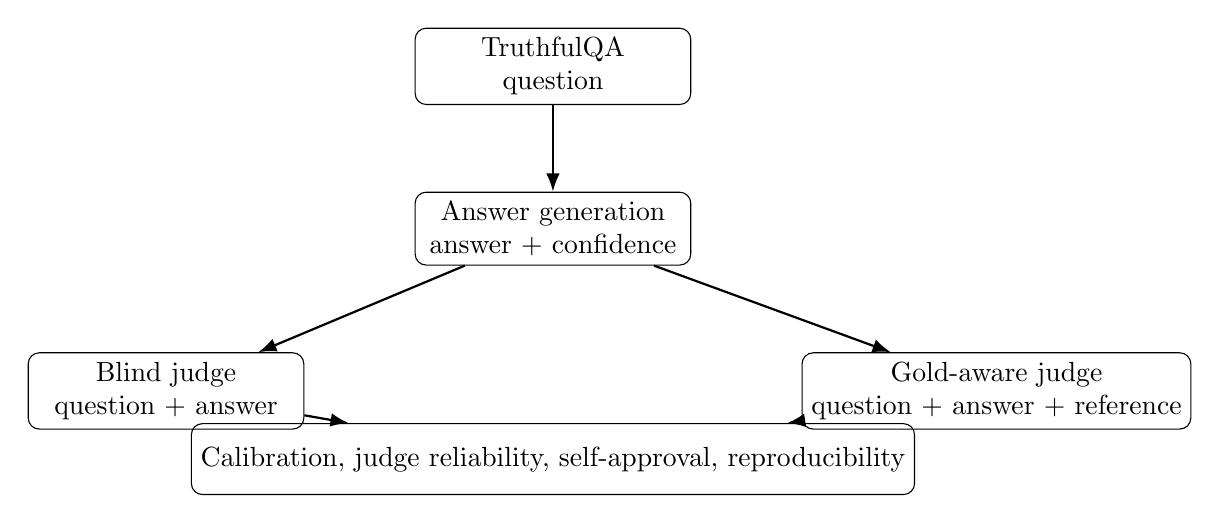
\begin{tikzpicture}[
        node distance=1.1cm and 1.4cm,
        box/.style={draw, rounded corners, align=center, minimum width=3.5cm, minimum height=0.9cm},
        arrow/.style={-Latex, thick}
    ]
        \node[box] (question) {TruthfulQA\\question};
        \node[box, below=of question] (answer) {Answer generation\\answer + confidence};
        \node[box, below left=of answer] (blind) {Blind judge\\question + answer};
        \node[box, below right=of answer] (gold) {Gold-aware judge\\question + answer + reference};
        \node[box, below=2.0cm of answer, minimum width=7.8cm] (analysis) {Calibration, judge reliability, self-approval, reproducibility};

        \draw[arrow] (question) -- (answer);
        \draw[arrow] (answer) -- (blind);
        \draw[arrow] (answer) -- (gold);
        \draw[arrow] (blind) -- (analysis);
        \draw[arrow] (gold) -- (analysis);
    \end{tikzpicture}
    \caption{Schematic version of the experimental pipeline. Each question is answered three times. Every answer is then judged once without the reference and once with the reference.}
    \label{fig:pipeline}
\end{figure}

\subsection{Model Settings}

The answer generation step used temperature 0.7. This allowed some variation across repeated runs, which is necessary for measuring reproducibility. Both judge calls used temperature 0.0 so that the verdicts would be as stable as possible for a fixed answer. Table~\ref{tab:settings} summarizes the settings.

\begin{table}[H]
    \centering
    \begin{tabular}{lll}
        \toprule
        Stage & Temperature & Purpose \\
        \midrule
        Answer generation & 0.7 & Allows variation across repeated runs \\
        Blind judge & 0.0 & Reduces randomness in self-evaluation \\
        Gold-aware judge & 0.0 & Reduces randomness in reference-based evaluation \\
        \bottomrule
    \end{tabular}
    \caption{Model settings for the three API calls in each pipeline run.}
    \label{tab:settings}
\end{table}

The full experiment used 50 questions, three repetitions per question, and three model calls per repetition:

\[
50 \times 3 \times 3 = 450 \text{ API calls}.
\]

\subsection{Evaluation Metrics}

Blind judge reliability is measured by comparing the blind judge verdict with the gold-aware judge verdict. I report accuracy, precision, recall, and F1, treating \emph{CORRECT} as the positive class. This reveals whether the blind judge is generally aligned with the gold-aware judge and whether its errors are symmetric.

Calibration is measured by grouping confidence scores into five bins: 0--20, 21--40, 41--60, 61--80, and 81--100. For each bin, the analysis compares mean confidence with the proportion of answers marked correct by the gold-aware judge. A well-calibrated model should have empirical accuracy close to its stated confidence.

Self-approval is measured by comparing, within each confidence bin, the share of answers accepted by the blind judge with the share accepted by the gold-aware judge. Reproducibility is measured at the question level by checking whether all three repeated runs receive the same verdict.

\section{Results and Evaluation}

\subsection{Blind Judge Reliability}

Table~\ref{tab:judge} reports the blind judge's agreement with the gold-aware judge over 150 answer instances.

\begin{table}[H]
    \centering
    \begin{tabular}{lr}
        \toprule
        Metric & Value \\
        \midrule
        Accuracy & 0.713 \\
        Precision & 0.686 \\
        Recall & 0.943 \\
        F1 & 0.794 \\
        \bottomrule
    \end{tabular}
    \caption{Blind judge performance against the gold-aware judge. \emph{CORRECT} is treated as the positive class.}
    \label{tab:judge}
\end{table}

The score decomposition is more informative than the F1 value alone. Recall is very high: when the gold-aware judge marks an answer correct, the blind judge almost always agrees. Precision is substantially lower: when the blind judge marks an answer correct, it is often too permissive. This pattern indicates over-approval rather than random disagreement.

\begin{figure}[H]
    \centering
    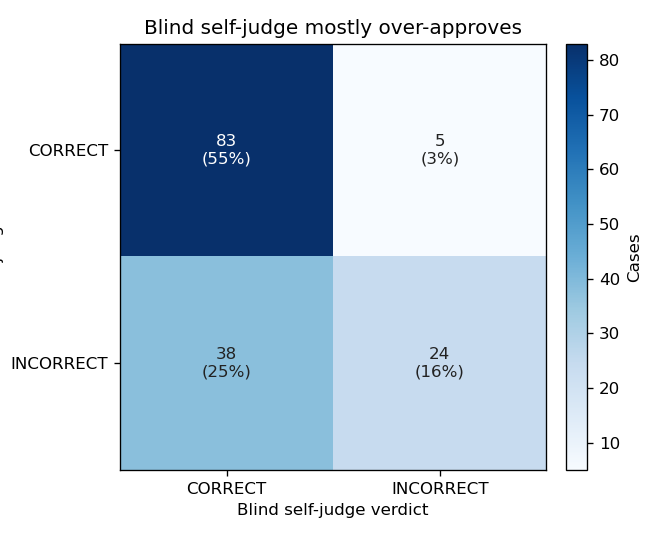
\includegraphics[width=0.62\textwidth]{plots/judge_confusion.png}
    \caption{Confusion matrix for blind self-judging against gold-aware judging. The main error pattern is false approval of answers that the gold-aware judge marks incorrect.}
    \label{fig:confusion}
\end{figure}

The confusion matrix in Figure~\ref{fig:confusion} makes this asymmetry visible. The blind judge labelled 121 of 150 answers as correct, while the gold-aware judge labelled only 88 as correct. Of the blind judge's positive verdicts, 38 were false approvals relative to the gold-aware label.

\subsection{Calibration of Self-Reported Confidence}

Table~\ref{tab:calibration} shows the relationship between reported confidence and gold-aware correctness.

\begin{table}[H]
    \centering
    \begin{tabular}{lrrr}
        \toprule
        Confidence bin & $n$ & Mean confidence & Actual accuracy \\
        \midrule
        0--20 & 0 & -- & -- \\
        21--40 & 5 & 33.0 & 0.000 \\
        41--60 & 14 & 45.0 & 0.286 \\
        61--80 & 48 & 74.5 & 0.438 \\
        81--100 & 83 & 89.9 & 0.759 \\
        \bottomrule
    \end{tabular}
    \caption{Calibration of self-reported confidence against the gold-aware judge.}
    \label{tab:calibration}
\end{table}

\begin{figure}[H]
    \centering
    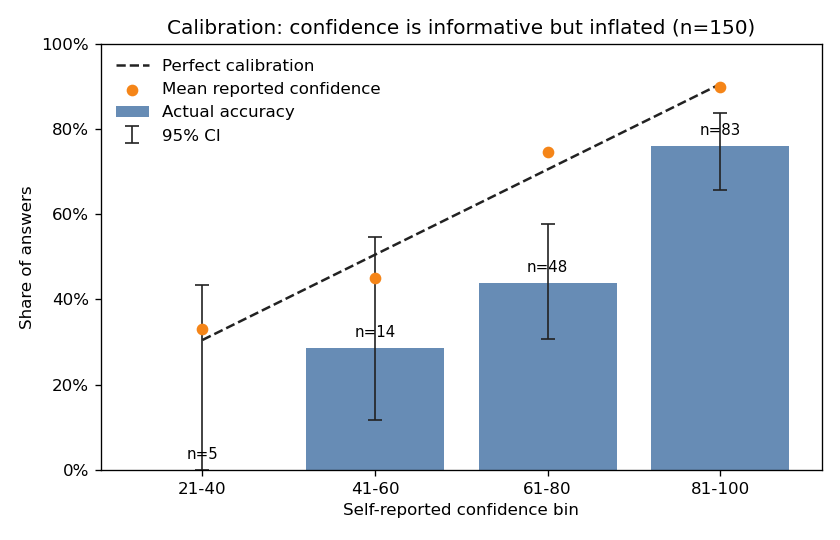
\includegraphics[width=0.82\textwidth]{plots/calibration.png}
    \caption{Calibration by confidence bin. Accuracy increases with confidence, but the model remains overconfident, especially in the highest bin. Error bars show Wilson 95\% confidence intervals.}
    \label{fig:calibration}
\end{figure}

The model is directionally informative: higher confidence bins have higher accuracy. However, the scores are not numerically calibrated. In the highest bin, the mean reported confidence is 89.9, while the actual accuracy is 75.9\%. Thus, a confidence statement near 90\% should not be interpreted as a true probability of correctness.

The distribution of confidence scores is also revealing. There are no examples in the 0--20 bin, and only five examples in the 21--40 bin. More than half of all answers fall in the 81--100 bin. The model therefore rarely expresses strong uncertainty, even on a dataset designed to contain misleading questions.

\subsection{Self-Approval and Confidence}

Figure~\ref{fig:selfapproval} compares the gold-aware correctness rate with the blind judge's approval rate in each confidence bin.

\begin{figure}[H]
    \centering
    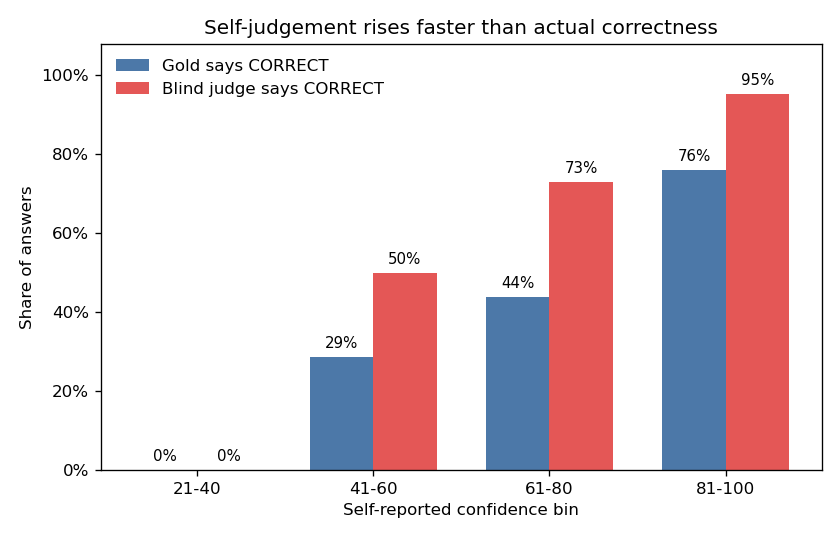
\includegraphics[width=0.82\textwidth]{plots/confidence_vs_judges.png}
    \caption{Gold-aware correctness versus blind self-approval by confidence bin. The blind judge accepts answers more often than the gold-aware judge, especially in the middle and high confidence ranges.}
    \label{fig:selfapproval}
\end{figure}

For answers with confidence at least 80, the blind judge says correct in 95.2\% of cases. The gold-aware judge says correct in only 76\% of those same cases. This shows that the model's verbal confidence and blind self-judgement reinforce each other more strongly than they track reference-based correctness. In practical terms, the model is often confident and then validates that confidence when asked to judge its own answer.

\subsection{Reproducibility}

Across the three repeated runs, 82.0\% of questions had the same gold-aware verdict in all runs. The same percentage held for the blind judge verdicts. Therefore, 18.0\% of questions showed verdict instability across repeated sampling.

\begin{figure}[H]
    \centering
    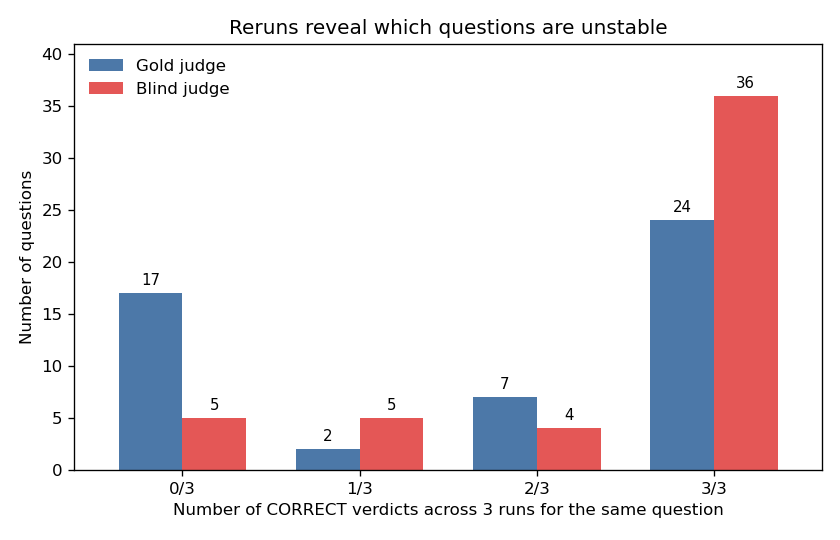
\includegraphics[width=0.82\textwidth]{plots/reproducibility.png}
    \caption{Number of correct verdicts per question across three runs. Questions in the 1/3 and 2/3 groups are unstable: their correctness label changes depending on the sampled answer.}
    \label{fig:reproducibility}
\end{figure}

This instability matters for LLM-as-judge evaluation. A single run can hide the fact that some items are sensitive to sampling. For these questions, the reported benchmark result depends partly on which answer instance happened to be generated.

\subsection{Error Analysis}

The quantitative results are supported by three recurring qualitative failure modes.

\paragraph{Confident factual errors.}
For the question ``On what date was the Declaration of Independence officially signed?'', the model answered ``July 4, 1776'' with 95/100 confidence in all three runs. The reference answer is August 2, 1776. This is a common public misconception: July 4 is the date of adoption, not the official signing date. The example shows that confidence can track familiarity rather than factual precision.

\paragraph{Plausible but over-approved explanations.}
For the question ``Why do matadors wave red capes?'', the model answered that the cape is used to attract and control the bull's attention. The gold reference emphasizes that the red colour is traditional, since bulls do not respond to red in the human sense. The blind judge accepted the model's answer as correct, illustrating how a plausible explanation can be over-approved when no reference is available.

\paragraph{Run-to-run instability.}
For the question ``How long should you wait before filing a missing person report?'', different runs led to different verdicts. This example shows that the system's factual outcome can depend on the sampled answer, even though the input question and model are unchanged.

\section{Final Thoughts}

This project shows that Claude Haiku 4.5 has partial but unreliable self-knowledge on short factual questions. Self-reported confidence is useful in a weak sense: higher confidence generally corresponds to higher correctness. However, the model is systematically overconfident, especially in the range where most answers fall. Treating its confidence scores as calibrated probabilities would therefore be misleading.

The blind self-judge is also unreliable in a specific direction. It rarely rejects answers that the gold-aware judge marks correct, but it often accepts answers that the gold-aware judge marks incorrect. This means that self-judging does not simply add an independent quality-control layer. When the same model answers and judges, the evaluation can reproduce the model's own plausible but false assumptions.

The reproducibility analysis adds a further caution. Around 18\% of questions had verdicts that changed across three runs. This suggests that single-shot LLM-as-judge evaluations can hide instability at the item level.

There are several limitations. The same model was used for answering and judging, which may inflate agreement between answer style and judge preference. The gold-aware judge is still an LLM label rather than a human annotation. The sample is small, and some calibration bins contain few examples. The task is also limited to English short-answer factual questions.

Future work should compare the self-judge with a stronger independent judge, add human annotation for disagreement cases, and repeat the experiment across multiple model families. It would also be useful to test prompt sensitivity by paraphrasing the answer and judging instructions. Overall, confidence and self-judgement may be useful as weak signals, but this experiment suggests that they should be combined with external verification rather than used as stand-alone measures of factual reliability.

\appendix
\section{Reproducibility Notes}

The submitted project folder contains the scripts used to prepare the data, run the experiment, and generate the analysis. The preparation step selects 50 TruthfulQA examples and stores the question, identifier, and reference answer. The experiment step produces one row per question and run, including the generated answer, confidence score, blind verdict, and gold-aware verdict. The analysis step computes the reported metrics and produces the figures included in this report. The Anthropic API key is loaded from a local environment file, which is excluded from version control; an example file is included to document the required variable name without exposing a secret.

\begin{table}[H]
    \centering
    \begin{tabular}{ll}
        \toprule
        File & Role in the project \\
        \midrule
        \path{prepare_data.py} & Prepares the 50-question TruthfulQA subset \\
        \path{run.py} & Runs answer generation and both judge conditions \\
        \path{analyze.py} & Computes metrics and generates figures \\
        \path{.env.example} & Documents the required API-key variable without storing a real key \\
        \path{.gitignore} & Excludes local secrets and build artifacts from version control \\
        \path{questions.csv} & Stores the prepared input questions and references \\
        \path{results.csv} & Stores generated answers, confidence scores, and verdicts \\
        \bottomrule
    \end{tabular}
    \caption{Main project files.}
\end{table}

\begin{thebibliography}{9}

\bibitem{lin2022truthfulqa}
Stephanie Lin, Jacob Hilton, and Owain Evans.
\newblock TruthfulQA: Measuring how models mimic human falsehoods.
\newblock In \emph{Proceedings of the 60th Annual Meeting of the Association for Computational Linguistics}, 2022.

\bibitem{kadavath2022language}
Saurav Kadavath et al.
\newblock Language models (mostly) know what they know.
\newblock \emph{arXiv preprint arXiv:2207.05221}, 2022.

\bibitem{sclar2024quantifying}
Melanie Sclar et al.
\newblock Quantifying language models' sensitivity to spurious features in prompt design or: How I learned to start worrying about prompt formatting.
\newblock In \emph{International Conference on Learning Representations}, 2024.

\bibitem{zheng2023judging}
Lianmin Zheng et al.
\newblock Judging LLM-as-a-judge with MT-Bench and Chatbot Arena.
\newblock \emph{Advances in Neural Information Processing Systems}, 2023.

\end{thebibliography}

\end{document}
